\chapter{Sistema de Reconhecimento Facial Visage} \label{chap:visage}

Intro ...


\section{Filtros de Abstração de Imagens no Reconhecimento Facial}
O reconhecimento facial em imagens sofreu uma evolução notável nos últimos 20 anos, tal como documentado no capítulo \ref{chap:reco} deste relatório. 

Em cenários cooperativos com condições de captura de imagens controladas, nomeadamente ao nível da pose, iluminação e expressões faciais, considera-se mesmo que o problema de verificação 1:1 se encontra praticamente resolvido, uma vez que as taxas de reconhecimento atingidas são satisfatórias para a grande maioria das aplicações \cite{Li2011}. Existem também várias aplicações em situações reais com um bom nível de satisfação por parte dos seus utilizadores, como é o caso do sistema de fronteira automático dos aeroportos portugueses (ver \ref{CartoesInteligentes}), ou o controlo de entradas nas cerimónias inaugurais dos jogos olímpicos de Pequim (ver \ref{sec:SegurancaAplicaçãoLei}). Em condições específicas e favoráveis, é então possível considerar que os sistemas de reconhecimento facial automático atuais conseguem mesmo ultrapassar a capacidade de reconhecimento humana, uma vez que conseguem identificar com precisão um maior número de faces do que aquelas que um humano consegue.

Contudo, o problema de reconhecimento facial automático ainda se encontra longe de ser um problema totalmente resolvido. Em cenários onde é registada uma grande variação ao nível da pose, iluminação ou outros fatores identificados na secção \ref{desafios} deste relatório, a identificação das entidades capturadas é ainda uma tarefa desafiante  \cite{Li2011}. Para além disso, a performance e satisfação obtida por parte dos utilizadores dos sistemas atuais demonstra uma grande variação tendo em conta as situações onde estes sistemas são utilizados. 

Por outro lado, a crescente ubiquidade tecnológica e poder computacional presente nos diversos dispositivos utilizados no nosso dia a dia, aumenta o leque de aplicações possíveis do reconhecimento facial automático, apresentando novos desafios às soluções de atualmente existentes.(ver \ref{sec:areasAplicacao})

Considerando todos os fatores mencionados anteriormente e ainda o elevado valor comercial das soluções existentes e consequente falta soluções abertas, torna-se pertinente a realização de investigação na área do reconhecimento facial em imagens. 

Ao nível da abstração de imagens, estudos efetuados demonstraram que aplicação destes filtros na recuperação de informação multimédia, nomeadamente no âmbito da da ilustração automática de texto têm a potencialidade de melhorar a informação retornada, assim como reduzir significativamente as necessidades de processamento e armazenamento das imagens \cite{Coelho:2012:IAC:2260641.2260676}. 

Tendo em conta a importância e a necessidade de investigação na área do reconhecimento facial automático, e uma vez que não existem estudos relativos à utilização de filtros de abstração no processo de reconhecimento facial, torna-se pertinente o estudo do seu impacto, no âmbito desta dissertação. Desta forma, a hipótese levantada no âmbito desta dissertação é então que o uso da abstração em imagens que vão ser ser alvo de reconhecimento facial pode melhorar o processo de reconhecimento facial automático em imagens.

\section{Coleção de dados} \label{sec:colecoes}

A evolução do estado da arte do reconhecimento facial automático em imagens tem beneficiado em larga escala do aumento constante dos recursos disponíveis para o seu estudo, nomeadamente através da criação de novas e mais completas coleções de dados \cite{Huang2007}. A grande maioria destas coleções, caracteriza-se por ter condições de captura controladas com o intuito de efetuar o estudo de fatores específicos que afetam a qualidade do reconhecimento, tais como a variação da pose, iluminação, expressão e outros fatores mencionados no capítulo \ref{desafios}. O objeto de estudo desta dissertação não é, no entanto, a análise específica de alguns desses fatores, mas sim a criação de um sistema de reconhecimento facial automático em imagens a partir de recursos de código aberto disponíveis, assim como a análise posterior do impacto do uso de abstração de imagens no sistema desenvolvido. Desta forma, a escolha de uma biblioteca apropriada e que represente as grandes variações associadas aos diferentes desafios que afetam o reconhecimento facial em imagens torna-se crucial.

Tendo em conta as preocupações acima mencionadas, para o desenvolvimento do sistema de reconhecimento facial  Visage e posterior análise dos resultados obtidos no âmbito nesta dissertação foi escolhida a coleção de imagens \textit{Labeled Faces in the Wild}. Esta coleção é constituída por um conjunto de imagens faciais e respetivas anotações textuais e encontra-se descrita em maior pormenor na secção seguinte deste documento.

\subsection{\textit{Labeled Faces in the Wild}}  \label{sec:lfw}
A coleção \textit{Labeled Faces in the Wild (LFW)} é uma base de dados fotográfica desenhada especificamente para o estudo do problema de reconhecimento facial, particularmente em situações onde as condições de captura das imagens não possuem restrições. Nesse sentido, as imagens que constituem a galeria caracterizam-se por possuir uma grande variabilidade, nomeadamente ao nível da pose, expressão, iluminação, etnia, idade, género, vestuário e qualidade da câmara, por exemplo \cite{Huang2007}.

Nesta coleção encontram-se representados um conjunto de 5749 indivíduos, ilustrados por 13233 imagens. O número de imagens por pessoa apresenta no entanto uma grande variação, desde um mínimo de 1 imagem por pessoa para 4069 indivíduos, até um máximo de 530 imagens que representam o antigo presidente dos Estados Unidos da América George W. Bush. O gráfico \ref{fig:distribuicaoLFW} ilustra a grande variação da distribuição do número de imagens por pessoa.

\begin{figure}[ht]
  \begin{center}
    \leavevmode
    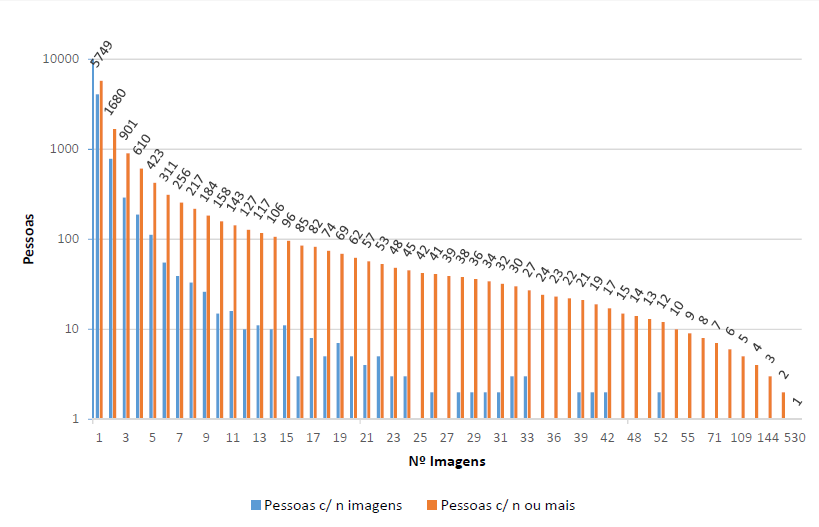
\includegraphics[width=1\textwidth]{Distribuicao}
    \caption{Distribuição do número de imagens por pessoa na biblioteca LFW. No eixo vertical encontram-se representadas o número de pessoas em escala logarítmica e no eixo horizontal o número de imagens correspondente.}
    \label{fig:distribuicaoLFW}
  \end{center}
\end{figure}

As imagens desta coleção são maioritariamente a cores, com diferentes graus de saturação, existindo também um número reduzido de imagens a preto e branco. Devido à inexistência de restrições na captura de imagens, cada fotografia pode possuir mais do que uma face representada, sendo que a face que contem o pixel central deve ser considerada como a entidade representada na imagem. A cada imagem encontra-se também associada uma anotação textual, relativa ao nome da pessoa representada. A tabela \ref{tab:lfw} sintetiza algumas das características mais significativas da biblioteca.

\begin{center}
\begin{table}
	\caption{Caracterização da Biblioteca LFW}
	\begin{center}
    \begin{tabular}{ll}
    \hline
    Característica                            & Valor            \\ \hline
    Imagens                                   & 13233 imagens    \\
    Pessoas representadas                     & 5749 pessoas     \\
    Tamanho total / Formato                   & 179 MB / JPEG    \\
    Tamanho de cada imagem: min / médio / max & ~                \\
    Dimensões imagem                          & 250 $x$ 250 pixeis \\
    \hline
    \end{tabular}
	\label{tab:lfw}
	\end{center}
\end{table}
\end{center}

Para além da coleção LFW original, encontram-se também disponíveis para fins de investigação duas outras coleções derivadas da coleção original, LFW funneled e LFW-a, onde as imagens originais foram sujeitas a um pré-processamento com vista a efetuar o alinhamento da posição da face na imagem, cada uma correspondendo a uma técnica diferente de alinhamento da imagem, respetivamente. Um exemplo dos resultados obtidos nas diferentes bibliotecas pode ser visto na figura \ref{fig:lfwversoes}.

- figura com três caras cada uma de um LFW diferente.

A coleção LFW é particularmente interessante para o estudo do desempenho do sistema desenvolvido e consequentemente do impacto do uso da abstração de imagens no reconhecimento facial uma vez que a variabilidade presente nas suas imagens, representa uma amostra fiável das variações encontradas no dia-a-dia de uma pessoa. Por outro lado, o facto de as suas imagens não terem sido capturadas com o intuito específico da análise do problema do reconhecimento facial, aproxima este conjunto de dados das imagens utilizadas por um utilizador final de um sistema de reconhecimento facial automático na grande maioria das situações. Finalmente, e uma vez que a tarefa de alinhamento da face na imagem não é um objeto de estudo primordial desta dissertação, a existência de versões já alinhadas da coleção permitiu agilizar os testes realizados, retirando um fator importante de variação dos resultados obtidos. Assim sendo, no âmbito desta dissertação optamos pela utilização da versão alinhada LFW-a \citep{autor} para fins de avaliação do desempenho do sistema de reconhecimento facial criado e do impacto do uso de filtros de abstração sobre essas imagens.

\section{Implementação}

\subsection{Sistema de Reconhecimento Facial Base - OpenCV Face Recognizer}
O \textit{OpenCV} é uma biblioteca de código aberto nas áreas de visão por computador e \textit{machine learning}, onde se encontra disponível a implementação de mais de 2500 algoritmos relacionados com as áreas de computação gráfica e visão por computador. Esta biblioteca possui uma comunidade de mais de 47 mil pessoas, já registou mais de 5 milhões de downloads e é utilizada globalmente por empresas como a Google, Yahoo, Microsoft, Intel, IBM, Sony, Honda, Toyota \cite{Team}. 

Ao nível do reconhecimento facial, esta biblioteca disponibiliza um módulo denominado \textit{Face Recognizer}, onde se encontram implementados os algoritmos \textit{Eigenfaces}, \textit{Fisherfaces} e \textit{Local Binary Patterns Histograms}.

Tendo em conta a ampla utilização da biblioteca OpenCV e a sua constante atualização pela comunidade, assim como as facilidades providenciadas pelo módulo de reconhecimento facial, esta foi considerada a biblioteca ideal para utilizar como base de implementação do sistema de reconhecimento facial a criar. De seguida encontram-se brevemente descritas as principais diferenças entre os três algoritmos implementados no módulo \textit{Face Recognizer:}

\subsubsection*{\textit{Eigenfaces}}
O método \textit{Eigenfaces} foi introduzido por Turk e Pentland em 1991 \cite{Turk1991}, e tira partido da Análise dos Componentes Principais (ACP) para efetuar o reconhecimento facial automático.

A análise de componentes principais tem como objetivo determinar as relações existentes entre diferentes conjuntos de dados, nomeadamente ao nível das suas diferenças e semelhanças, tirando partido da redundância existente para criar uma representação reduzida dos dados sem que a perda de informação ocorrida seja significativa. As imagens faciais possuem uma grande redundância natural, o algoritmo \textit{Eigenfaces}, através da análise dos componentes principais dessas imagens, efetua uma projeção das imagens faciais num sub-espaço onde se evidenciam apenas as variações entre as diversas caras conhecidas pelo sistema.

A redução do espaço de representação revela-se fulcral no problema de reconhecimento facial em imagens, devido à grande dimensionalidade exigida para a representação de uma face. Considerando, por exemplo, uma dada imagem de $n$ x $m$ \textit{pixels} de tons cinzentos, essa imagem poderia ser traduzida por um espaço vetorial de $m = $ $n$ x $m$ \textit{pixels}, assim sendo, uma imagem de apenas $256x256$ \textit{pixels} necessitaria de um total de $65536$ \textit{pixels} para ser representada.

O processo de reconhecimento facial com recurso ao algoritmo \textit{Eigenfaces} consiste nos seguintes passos:
\begin{enumerate}
\item Aquisição de um conjunto de dados iniciais (conjunto de treino);
\item Projeção dos dados obtidos num sub-espaço de faces através da ACP;
\item Aquisição de uma imagem a reconhecer;
\item Projeção da face a reconhecer no sub-espaço do conjunto de treino, calculando as distâncias obtidas para cada face conhecida pelo sistema;
\item Determinar qual a face do conjunto de treino com menor distância à face a reconhecer;
\item Caso a distância para a face obtida seja menor do que um limite operacional estabelecido, a imagem é reconhecida como sendo essa pessoa, caso contrário, a face é identificada como sendo uma pessoa desconhecida pelo sistema.
\end{enumerate}

Este método efetua assim uma abordagem holística ao problema de reconhecimento facial em imagens, uma vez que tem em consideração a representação facial como um todo, não fazendo a distinção entre pontos específicos da face como olhos, orelhas ou nariz para efetuar o reconhecimento facial. Uma vantagem deste tipo de representação é a reduzida sensibilidade ao ruído presente nas imagens \cite{Zhao2003}.

\subsubsection*{\textit{Fisherfaces}}
A análise dos componentes principais visa determinar o sub-espaço onde se verifica uma maior variação entre um conjunto de imagens. No entanto, a variação na representação facial de uma pessoa encontra-se muitas vezes relacionada com mudanças de expressões faciais ou iluminação dos indivíduos, pelo que, o sub-espaço criado pelo algoritmo \textit{Eigenfaces} não traduz muitas vezes apenas as diferenças de identidade entre os diversos indivíduos, mas também as diferenças verificadas entre as várias representações de um indivíduo devido à variação nas condições de captura das imagens. O algoritmo \textit{Fisherfaces} \cite{Belhumeur1997, Etemad1997, Zhao1998}, tenta resolver este problema, através da aplicação de um passo de Análise Linear Discriminante (ALD) \textit{(Linear Discriminant analysis)} após a análise dos componentes principais, de forma a determinar mais corretamente as variações intra-classe existentes no conjunto de imagens a avaliar.

A ALD, inicialmente introduzida por Fisher em 1936 \cite{FISHER1936}, tenta maximizar as diferenças existentes entre diferentes indivíduos(inter-classe) e minimizar as variações entre imagens da mesma pessoa(intra-classe) de modo a obter uma representação mais robusta em termos de variação ao nível da iluminação. Após a aplicação dos passos de ACP e ALD, o processo de reconhecimento do método \textit{Fisherfaces} é semelhante ao efetuado pelo método \textit{Eigenfaces}, sendo também efetuada uma abordagem holística ao reconhecimento facial.


\subsubsection*	{\textit{Local Binary Patterns Histograms (LBPH)}}
Ao contrário dos algoritmos descritos anteriormente, o LBPH efetua uma abordagem local ao problema de reconhecimento facial, efetuando uma extração das características locais de uma imagem. Este tipo de abordagem possuí a vantagem de possuir uma baixa dimensionalidade implícita, pelo que não existe a necessidade de efetuar a projeção das imagens num sub-espaço.

A ideia base das \textit{Local Binary Patterns (LBP)}, consiste em resumir a estrutura local de imagem através de uma comparação de um pixel com os seus vizinhos. Dado um pixel central é analisada a diferença entre esse pixel e cada um dos seus vizinhos. Se a intensidade do pixel for maior ou igual do que a do seu vizinho é atribuído o valor 1, caso contrário é atribuído o valor 0. Cada pixel pode então ser traduzido por um número binário do género $11001111$. Dados $8$ pixeis é então possível efetuar $2^8$ combinações, cada uma designada de LBP.

Ahonen \textit{et al.} \cite{ahonen2004face}, propuseram o uso de LBP para o reconhecimento facial em imagens. A sua abordagem consiste na divisão da face em pequenas regiões das quais são derivadas LBP e concatenas numa representação única designada de LBPH, a qual representa uma imagem facial. O reconhecimento é depois efetuado através do determinação do vizinho mais próximo no espaço de faces computado.

\subsection{Filtros de Abstração - Filtro Kuwahara Anisotrópico}
\begin{figure}[ht]
  \begin{center}
    \leavevmode
    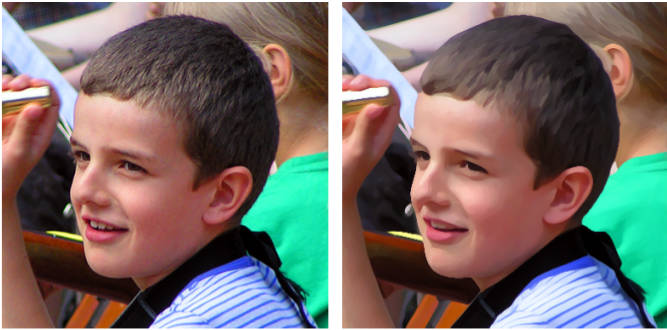
\includegraphics[width=0.7\textwidth]{filterskid}
    \caption{Comparação entre imagem não abstraída (esquerda) e imagem abstraída (direita) \cite{Kyprianidis2009}.}	
    \label{fig:filterskid}
  \end{center}
\end{figure}

Ao nível dos filtros de abstração o estudo será efetuado utilizado o filtro Kuwahara Anisotrópico (FKA).

Este filtro consiste numa generalização do filtro Kuwahara (ver \ref{subsec:kuwahara}) que remove alguns artefactos originados na aplicação do filtro original através da adaptação da forma, escala e orientação do filtro à estrutura local das características da imagem \cite{Kyprianidis2009}. Desta forma é produzido um efeito de abstração tipo pintura, onde é removida informação não essencial em zonas de elevado contraste, enquanto são preservados os limites representados nas zonas de menor contraste, tal como demonstrado na figura \ref{fig:filterskid}. As imagens ficam assim com a clareza de uma ilustração, mas preservam a informação direcional tal como nas pinturas a óleo clássicas. Por outro lado, este filtro tira partido da placa gráfica para a realização da abstração das imagens, tornando-se assim particularmente indicado para o processamento de um elevado número de fotografias.

O filtro em questão foi também utilizado anteriormente, e com resultados positivos, em abstração de imagens para a recuperação de informação multimédia. 

Tendo em conta os fatores apresentados consideramos que este filtro é o mais adequado para a utilização no âmbito deste projeto.
	
\section{Arquitectura}

	diagrama com a pipeline
	
	descrição dos módulos
	
\section{Detalhes Implementação}
...

\begin{figure}[ht]
  \begin{center}
    \leavevmode
    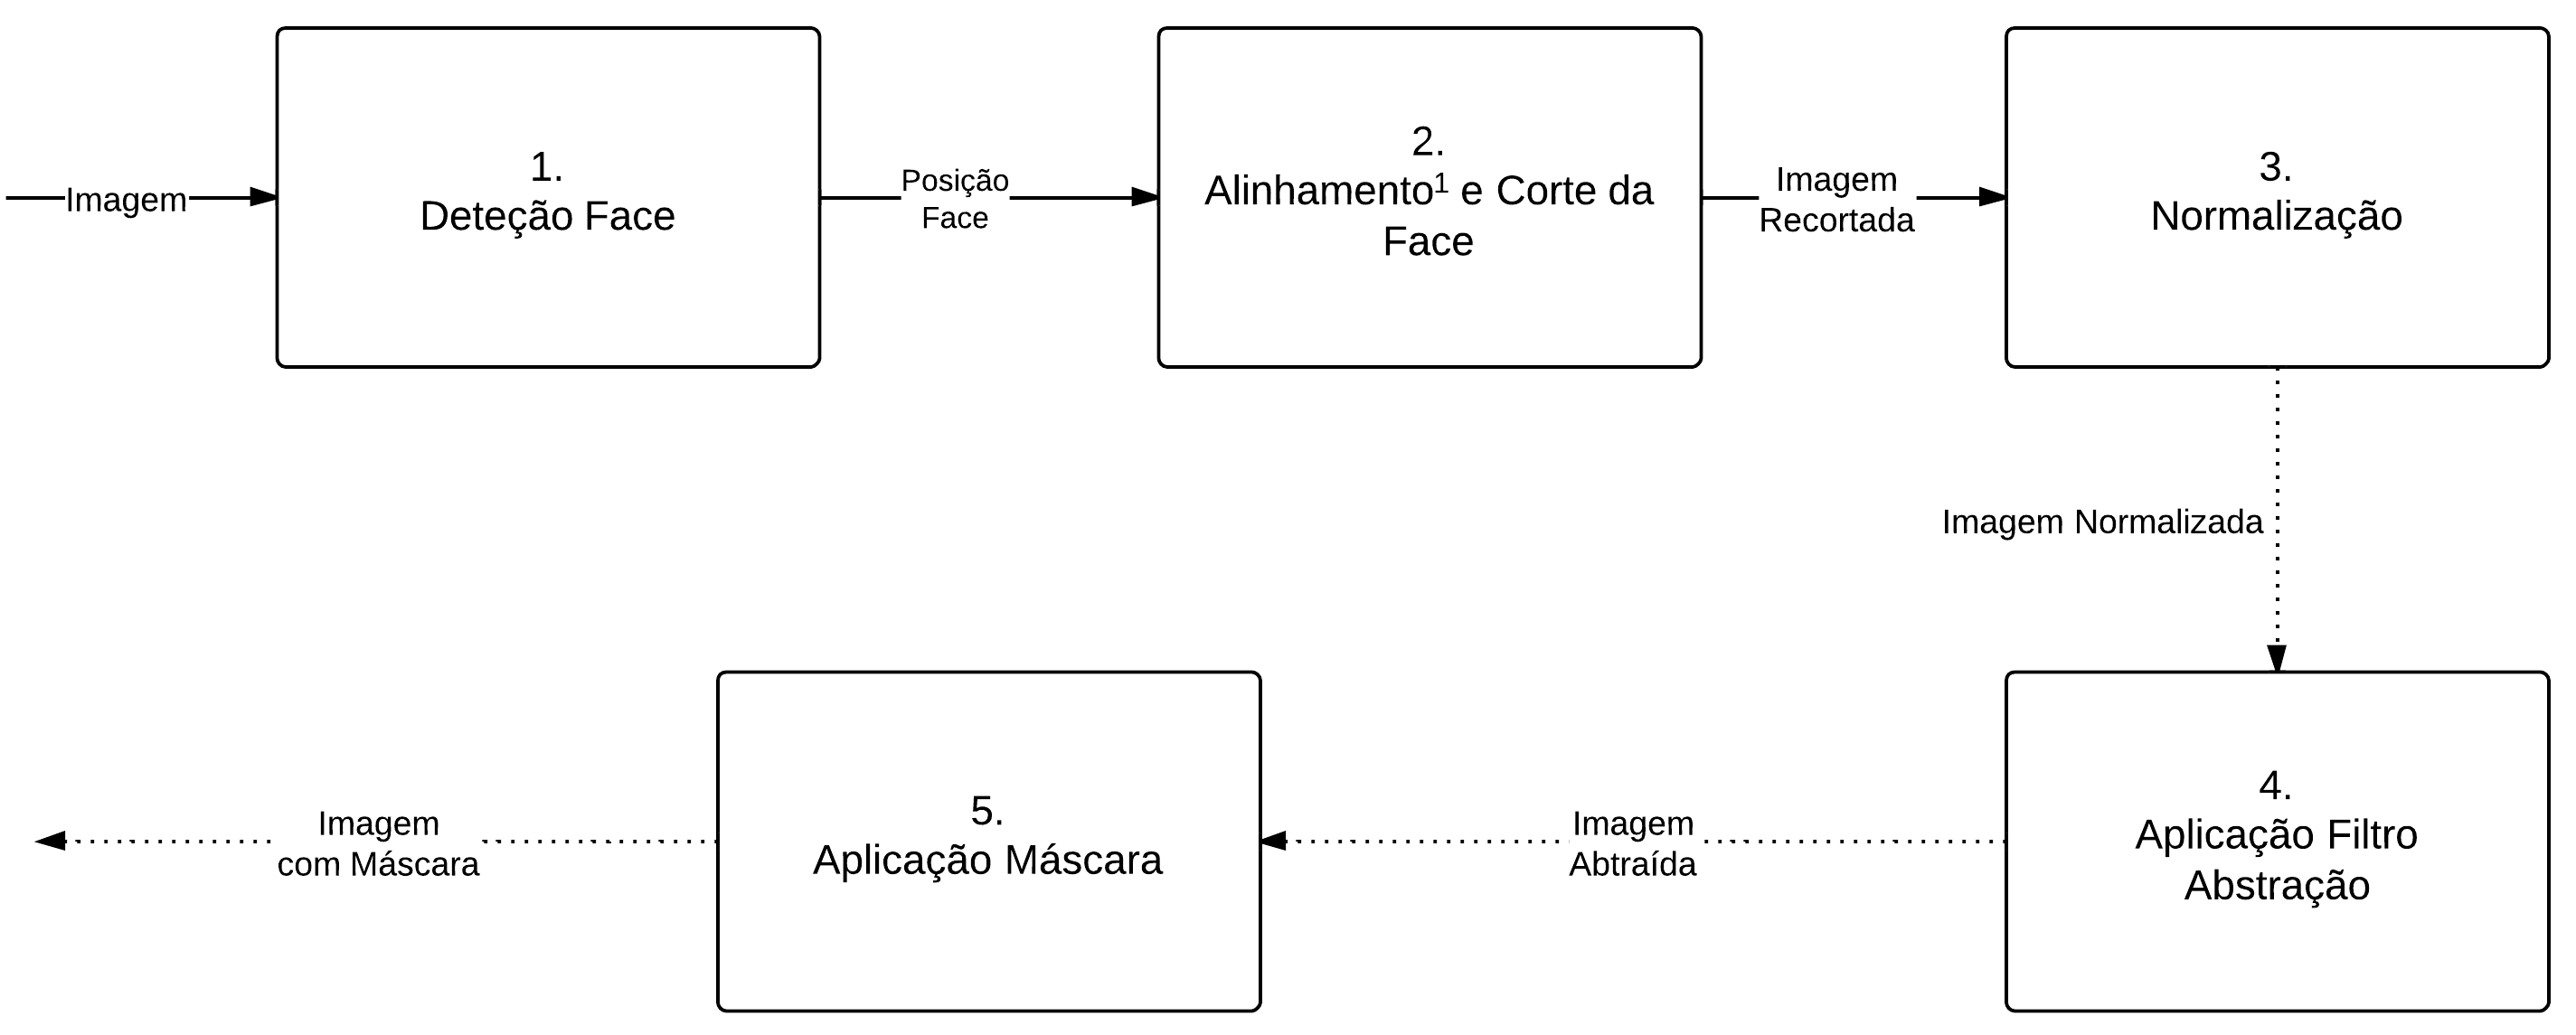
\includegraphics[width=0.7\textwidth]{PreProcessamentoVisage}
    \caption{Cadeia de pré-processamento a que as imagens podem ser sujeitas.}
    \label{fig:preprocessamento}
  \end{center}
\end{figure}

O passo 1 é responsável pela deteção da localização da face na imagem e efetuar a respectiva segmentação da mesma, de acordo com descrito em \ref{chap:detector}. Após a obtenção da face extraída da imagem é então possível proceder à sua normalização em termos de contraste. Para isso foram analisadas três possibilidades: \textit{contrast streching}, \textit{histogram equalization} e ainda \textit{CLAHE}. Posteriormente a imagem po....


\section{Funcionalidades}

	API?
